\documentclass{article}
\pdfpagewidth=8.5in
\pdfpageheight=11in

\usepackage{ijcai19}

% Use the postscript times font!
\usepackage{times}
\usepackage{soul}
\usepackage{url}
\usepackage[hidelinks]{hyperref}
\usepackage[utf8]{inputenc}
\usepackage[small]{caption}
\usepackage{graphicx}
\usepackage{amsmath}
\usepackage{booktabs}
\usepackage{tocloft}
\usepackage{url}
\urlstyle{same}

% dot leaders for section entries in table of contents
\renewcommand{\cftsecleader}{\cftdotfill{\cftdotsep}}

\newcommand{\etal}{\textit{et al.}}

\title{Is attention really all you need?}

\author{
Kyle Roth\\
\affiliations
Brigham Young University\\
\emails
kylrth@gmail.com
}

\begin{document}

\maketitle

\tableofcontents

\vspace{30px}

\begin{abstract}
This is a wonderful abstract.
\end{abstract}

\section{Introduction}

The attention mechanism is an exciting development in the artificial intelligence community. The concept is simple, and rooted in our understanding of attention in biological intelligence \cite{glimpses,neuroscience-inspired}. Attention mechanisms also lend themselves to more intuitive interpretation, an attractive feature as concerns about model interpretability gain traction. In this review, we observe the trajectory that current research is taking with regard to the theory and application of attention, and suggest how future work should try to understand why attention is so useful for such varied applications.

\subsection{Background on neural machine learning}\label{section:background}

Machine learning is a branch of artificial intelligence that deals with training a model to perform tasks by providing the model with data. There are various types of machine learning algorithms, applicable to different tasks. One of the most popular algorithms is the neural network. A neural network is a system of connections between simple functions (e.g. multiplication, summation, ReLU \cite{relu}), which together approximate a larger, more complex function. It has been proven that sufficiently large neural networks can approximate arbitrary continuous functions \cite{universal_approximators}. Theoretically, this means that for every reasonable mapping there exists a neural network that replicates it. Some example mappings are listed in Table~\ref{table:mappings}.

\begin{table}
    \centering
    \begin{tabular}{|c|c|}
        \hline
        \textbf{Input} & \textbf{Output} \\
        \hline
        images & the objects the image contains \\
        \hline
        audio recordings & a text transcription \\
        \hline
        English text & a French translation \\
        \hline
    \end{tabular}
    \caption{Mappings that a neural network can theoretically learn. Mappings must be consistent; that is, each input should only have one corresponding output.}\label{table:mappings}
\end{table}

Most commonly, neural networks undergo supervised training, meaning that they are shown the correct output for each training example and made to improve in some way. Neural networks generally use backpropagation\footnote{\textit{Backpropagation} refers to the calculation of the gradient for each trainable weight in the network. See \cite{backprop_theory} for details on backpropagation.} and gradient descent\footnote{\textit{Gradient descent} is a method of training wherein the weights are updated in the direction opposite the gradient at each training step \cite{gradient_descent}.} to train weights that are present in the simple functions of the network. Backpropagation uses the difference between the correct example and the network's output to determine how the weights in the network need to change. Figure~\ref{figure:backpropagation} provides a visualization of backpropagation in a neural network.

\begin{figure}
    \centering
    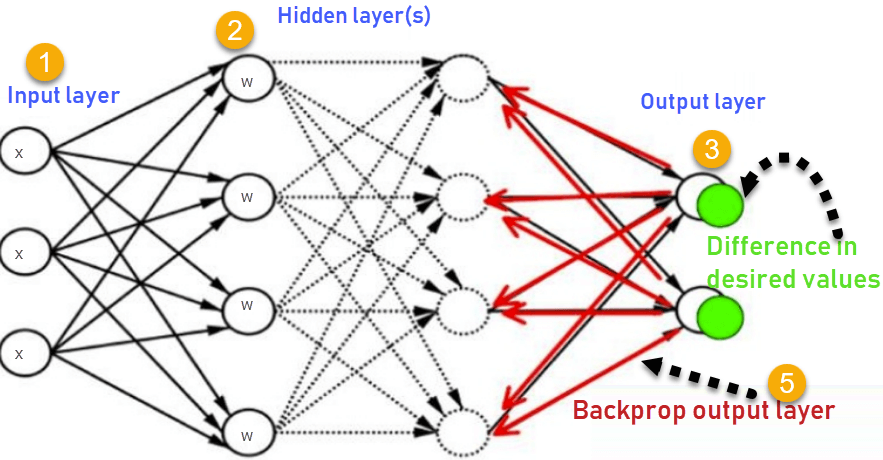
\includegraphics[width=3in]{figures/backpropagation.png}
    \caption{A visualization showing that backpropagation uses the difference between the desired and actual output to train the weights of the neural network. Image source~\protect\cite{backprop}.}\label{figure:backpropagation}
\end{figure}

While the theoretical limitations of neural networks are quite permissive, it is relatively difficult to train them. Backpropagation is sensitive to ``noisy'' or incorrect data, meaning that data cleaning and preparation is at least as important as architecture selection. The training process is also relatively expensive in terms of computation time and memory usage; neural networks are commonly trained for days or even months \cite{attn_all_you_need}.

Another real issue is that backpropagation is unlikely to find the ``global optimum'', the absolutely optimal set of weights that approximate the function. This is due to the fact that the algorithm only adjusts the weights incrementally, and can get stuck in a ``local optimum'', a condition where no slight change would improve performance but performance is still not as good as at the global optimum.

These difficulties with training neural networks are the reason that so much effort is given to developing better network architectures. Certain architectures and data representations lend themselves to a smoother search space for the weights, increasing the likelihood that backpropagation reaches a better optimum.

\subsection{Description of attention}

Attention appears to provide that smoother search space for training the network because its output can explicitly depend on each input given to the network, while also giving an intuitive view of the inputs that the network learns to ``attend'' to.

Bahdanau \etal~[\citeyear{joint_align_translate}] first described attention as an ``alignment model'' for words in a sentence to be translated. They used an RNN encoder-decoder model as others had before \cite{encoder_decoders}, but for every position in the target sentence, the alignment model produced a ``soft alignment''\footnote{In machine translation, \textit{alignment} refers to the pairing of words or phrases in the source sentence with words or phrases in the target sentence.} between the target location and every word in the source sentence. See Figure~\ref{figure:rnn_search} for more details on the model.

The key development here was the use of a soft alignment, meaning that each pair of source and target words was given an alignment score between 0 and 1. This made the alignment calculation differentiable\footnote{\textit{differentiable} means that the function has a derivative, allowing gradients to pass through with backpropagation.}, allowing the alignment to be performed by a feed-forward\footnote{\textit{Feed-forward} refers to the fact that all layers of the network produce output in the forward direction (as opposed to an RNN, for example, in which some output from a network is used as input to the same layer). An example representation can be seen in Figure~\ref{figure:backpropagation}.} neural network trained along with the rest of the model.

\begin{figure}
    \centering
    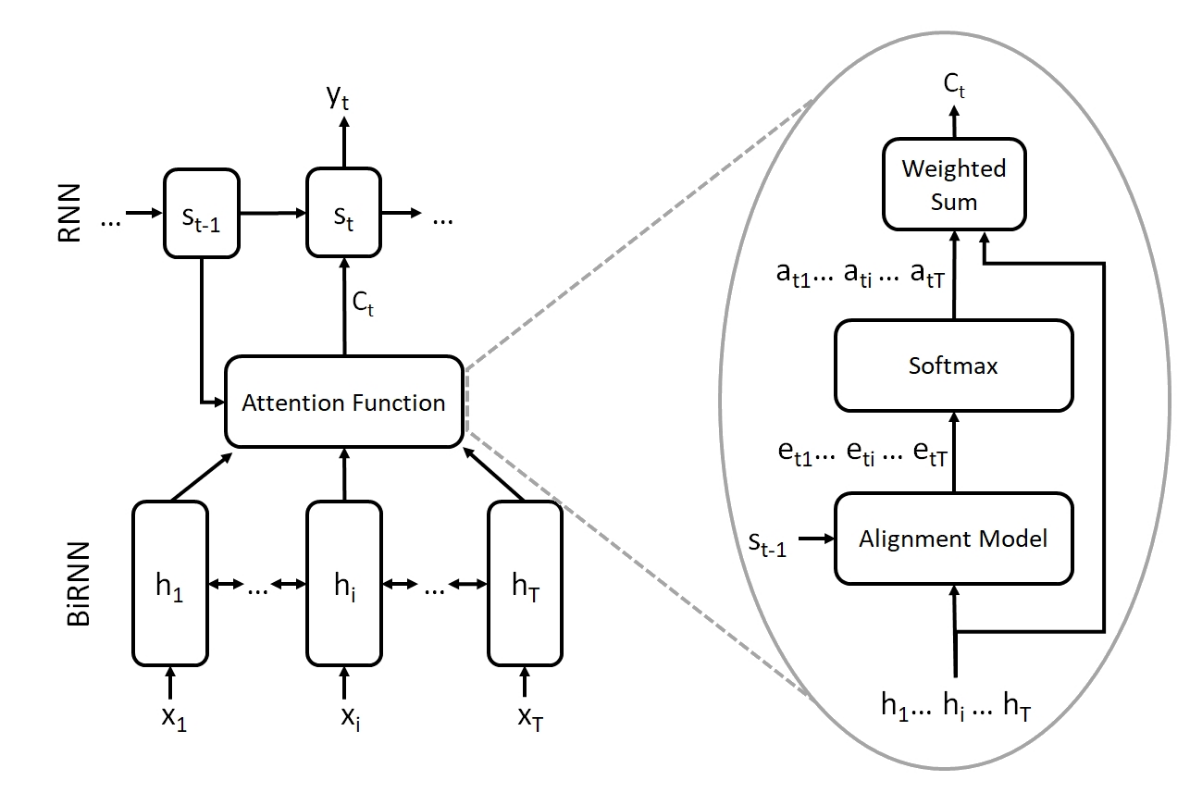
\includegraphics[width=3in]{figures/rnn_search.png}
    \caption{The model used by \protect\cite{joint_align_translate}. They used a bidirectional RNN to encode each word $x_i$ into a fixed-length vector $h_i$. Then, for every position $t$ in the target sentence, the alignment model produced an alignment vector $a_t$, a measure of alignment between the target location and every word in the source sentence. $a_t$ was used to find the weighted sum $c_t=\sum_{i=1}^Ta_{ti}h_i$, which was used as the input to the decoder (a unidirectional RNN). Note that the alignment model also received the previous decoder RNN state $s_{t-1}$ as input. Image source~\protect\cite{attention_please}.}\label{figure:rnn_search}
\end{figure}

\section{Theoretical generalization}

Ironically, attention mechanisms have received lots of attention since their conception in \citeyear{joint_align_translate}. Initially formulated as a word alignment mechanism for text translation \cite{joint_align_translate}, attention can be generalized in two ways: first in terms of the objects it operates on, and second in terms of the information it provides.

% \cite{listen_attend_spell}

% Unsure: \cite{show_observe_tell}, \cite{draw}

\subsection{Objects of attention}

There is a wide range of relationships that attention mechanisms can model. Specifically, we will see that attention has been generalized to include relationships between two input sequences, relationships within a single sequence, and relationships between arbitrary graphs. This generalization leads us to view attention beyond the scope of what the word ``attention'' implies.

\subsubsection{Inter-sequence attention}

Instead of applying attention to elements of an input sequence to predict an output sequence, Parikh \etal~[\citeyear{natural_language_inference}] successfully used an attention mechanism to produce relationships between elements of two input sequences. They successfully used this mechanism to perform natural language inference\footnote{\textit{Natural language inference} is the task of determining whether the meaning of a sentence entails (implies) or contradicts the meaning of another.}. Figure~\ref{figure:inference} makes it obvious that the attention function $F$ is determining the strength of the relationship between its two input words; that strength is used by the model to determine the entailment relationship of the pair of sentences.

\begin{figure}
    \centering
    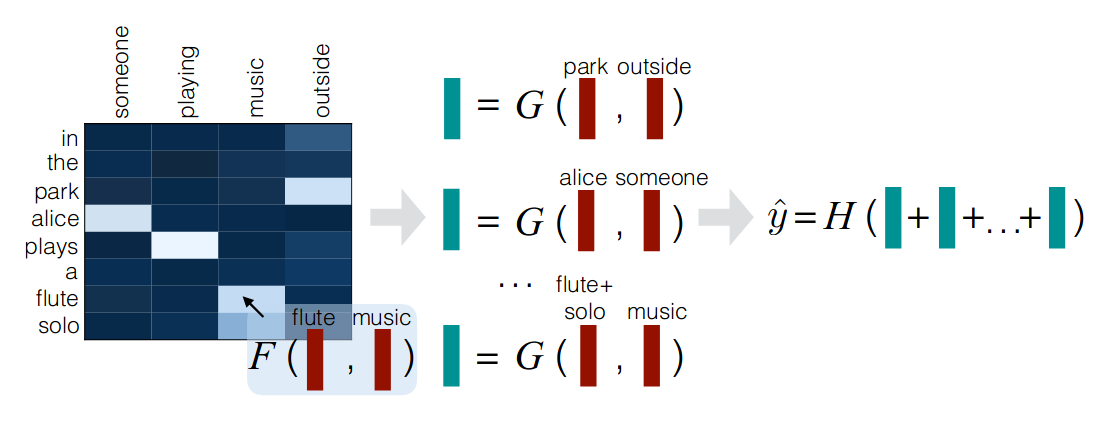
\includegraphics[width=3in]{figures/inference.png}
    \caption{The model used by \protect\cite{natural_language_inference}. $F$ is the attention model used to ``decompose the problem into the comparison of aligned subphrases''. $G$ compares the aligned subphrases. Both $F$ and $G$ were feed-forward networks in the work.}\label{figure:inference}
\end{figure}

\subsubsection{Self-attention}

Parikh \etal~[\citeyear{natural_language_inference}] also suggest what they term ``intra-sentence attention'' to represent relationships between words within the same input sentence. This is more broadly referred to as self-attention \cite{self_attentive_embedding,attn_all_you_need}. As the name suggests, self-attentive mechanisms learn the relationship between elements of a single sequence. While RNNs are theoretically able to do this, they struggle with long-distance relationships because they encode all relationships into a single context vector \cite{joint_align_translate}. Self-attention overcomes this difficulty, and provided for additional accuracy in the NLI model developed by Parikh \etal~[\citeyear{natural_language_inference}].

\subsubsection{Attention on arbitrary graphs}

Attention can also be used on more complex structures than sequences. Kim \etal~[\citeyear{graphs}] show that attention can be generalized to represent relationships between elements of arbitrary graphs\footnote{A \textit{graph} in this context refers to a set of elements with connections drawn between them. A sequence is a graph with elements connected one after the other, but in general a graph's elements can be connected to each other arbitrarily.}. This allows the model to accept parse trees and other useful structures that explicitly encode relationships in the data.

This use of attention is relevant because it blurs the line between data and relationships. In the case of Kim \etal~[\citeyear{graphs}], some known relationships were provided to the model in the form of parse tree structures. When the model was provided with this structure, the model learned to attend to entire subtrees as well as individual words. Thus the structure introduced in the data served as a way for the model to recognize and learn from information in the structural bias. Thus it was shown that attention mechanisms can learn from the inherent structure of their input.

More work should be given to understanding how attention learns from the structure of the objects it operates on. If attention can learn from the structure as well as the values of its input, any current application of attention could benefit from preprocessing the data to expose structural information. We've already seen this applied to natural language tasks \cite{graphs}, but structure could be extracted from images, videos, and longer-form text input like paragraphs or web pages.

\subsection{Information provided by attention}

Discovering the hidden biases\footnote{A \textit{bias} refers to the tendency of a network structure to exhibit a certain behavior, regardless of the weights the network. Understanding the biases of a network structure allows us to understand how it learns, and helps us predict strengths and weaknesses. See the last paragraph of Section~\ref{section:background} for a discussion of this aspect of neural network research.} of neural network models is an area of ongoing research in neural machine learning. Fortunately, much effort has been given to discovering the biases of attention models. Some limitations of attention have already been discovered, but others have only been hinted and and deserve further work.

\subsubsection{Active memory}

One of the first applications of attention was to create a completely differentiable neural Turing machine\footnote{In computing theory, a \textit{Turing machine} is any computer that can execute an arbitrary algorithm \cite{wiki:turing}.} \cite{neural_turing}. The model was given memory to read from and write to at each iteration, and an attention mechanism allowed those operations to be differentiable. Just as vanilla neural networks have been shown to approximate arbitrary functions, the neural Turing machine can approximate arbitrary programs.

One of the shortcomings of the neural Turing machine is that the attention mechanism is biased toward attending to one value more than any other \cite{active_memory}. Thus it is difficult to train the network to perform tasks requiring the model to read from multiple entries in memory, like adding two numbers. Kaiser and Bengio [\citeyear{active_memory}] suggested that attention suffers from exactly this issue, and offer a mechanism called active memory that attends to all inputs equally. They called their model the extended neural GPU, and it achieved promising results with better performance at translating long sentences. This could be due to the fact that long sentences are more likely to contain alignments that aren't one-to-one.

This appeared to be a promising generalization of attention, but the performance of the extended neural GPU was outstripped by later attention models that solved the single-focus problem using multi-headed attention \cite{attn_all_you_need} (see section~\ref{section:multi_headed}).

\subsubsection{Attention as a lookup mapping}

\begin{figure}
    \centering
    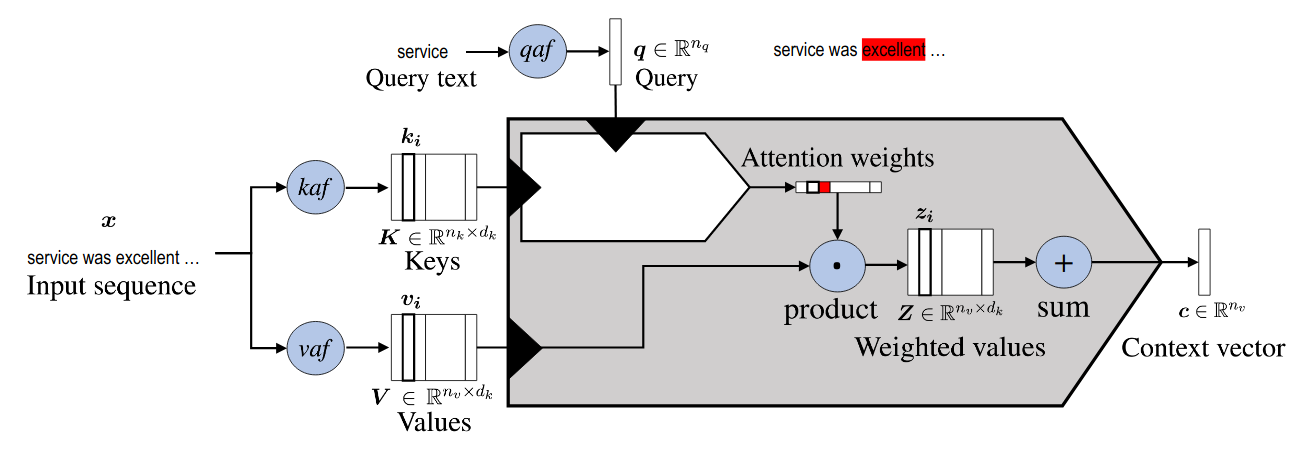
\includegraphics[width=3in]{figures/queries_keys_values.png}
\caption{The generalized model of attention from \protect\cite{attention_please}. Here $kaf$ and $vaf$ are functions mapping the input sequence to keys and values, respectively. An important distinction should be made between the terms ``attention weights'' and ``context vector'': attention weights are the ``soft alignment'' between the query and elements of the input sequence, and the context vector is the compiled information resulting from the weighted average of the values with respect to the attention weights. Image source~\protect\cite{attention_please}.}\label{figure:queries_keys_values}
\end{figure}

Several papers describe attention as a map from a sequence of keys to a sequence of context vectors, with exposure to queries and values \cite{attn_all_you_need,attention_please}. This model of attention makes no assumption about the type of input to the queries, keys, or values. The keys and values can be seen as different representations of the same input \cite{attention_please}, while the queries correspond to the current position of interest. See Figure~\ref{figure:queries_keys_values} for more details on this model of attention. The greatest difference between this model and the original from Bahdanau \etal~[\citeyear{joint_align_translate}] is the distinction between keys and values; Bahdanau \etal's model uses the same representation $h$ for both.

This unified model generalizes the mechanism to include nearly all forms of attention found in literature. It describes commonalities between all variants of the mechanism, and offers the possibility of more completely describing the functionality. More effort is needed to describe some of the biases and uncover the basic functionality of attention in greater detail.

\section{Application}

Here we review several recent applications of attention, observing common strengths and deficiencies. We also discuss directions that future work may take, given the strength that attention has shown in producing relationship metrics.

\subsection{Scaled dot-product attention}

With the original form of attention developed by Bahdanau \etal [\citeyear{joint_align_translate}], the relationship between the $j$th input representation $h_j$ and the $i$th output representation (query) $s_i$ can be represented as
\[
\text{attention}(h_j,s_i)=\left<v_j,a(W_1h_j+W_2s_i)\right>\text,
\]
where $\left<\cdot,\cdot\right>$ is a dot product\footnote{a weighted sum}, $v_j$ is the value representation, $a$ is an activation function\footnote{An \textit{activation function} is a non-linear function typically used at the output of a neural network, so that it can learn non-linear mappings.}, and $W_1,W_2$ are trainable weight matrices \cite{massive_exploration}.

Luong and Manning [\citeyear{multiplicative_attn}] introduced a modified mechanism that's faster and produces nearly the same performance. It is called \textit{multiplicative attention}, in contrast with the original \textit{additive attention} \cite{massive_exploration}. Multiplicative attention is defined as
\[
\text{attention}(h_j,s_i)=\left<W_1h_j,W_2s_i\right>\text,
\]
which ignores the value representation $v_j$. Additive attention ``slightly but consistently outperformed'' multiplicative attention in a battery of tests \cite{massive_exploration}, but the speed benefit of multiplicative attention is attractive enough that many later models used that implementation \cite{attn_all_you_need,more_multiplicative}.

\subsection{Attention without weights}

Vaswani \etal~[\citeyear{attn_all_you_need}] further simplified the computation of attention by removing the learned weights $W_1$ and $W_2$

\subsection{Attention without recurrent layers}

\cite{attn_all_you_need}

\cite{attn_all_you_need}

\subsection{Multi-headed attention}\label{section:multi_headed}

\cite{attn_all_you_need}

\subsection{Model interpretation}

Given that attention mechanisms learn relationships between sequences, we wonder if a simpler mechanism could learn the relationship from many inputs to a single output. One of the drawbacks of neural networks is that they don't provide a way to create feature importance metrics. These metrics are useful for determining why a model makes the decisions it does. In many papers cited here, attention produces a relationship matrix that provides intuition about the model's reasoning. It's possible that that same matrix could be produced by a simpler attention mechanism focused on the features that contribute to a single output value.

\section{Conclusion}

Currently, what is known for certain is that attention is useful. What is not known is exactly what it provides to the model. Is it simply a good way to generate a context vector, or does it successfully encode all the information needed to produce the output? Is it simply a limited version of something more powerful?

\bibliographystyle{named}
\bibliography{main}

\end{document}
